En person står på en lina som är uppspänd mellan två bergskanter. När personen påverkas av en kraft uppstår svängningar i linan.
Man skulle exempelvis kunna påverka personen med krafter genom att ge denne vikter eller heliumballonger. Alternativt skulle personen kunna böja på sin ben vilket skulle skapa andra svängningar i linan.
Hur linan kommer svänga beror på många variabler till exempel personens vikt, linans längd, var på linan personen står och materialet som linan är gjord av. 

Det kan vara svårt säga hur linan kommer svänga beroende på vilka av de ovanstående händelserna som sker.
För att kunna beskriva detta fysikaliskt kommer vi skapa en modell (se Figur \ref{fig:skiss}) 
för svängningssystemet som ett linjärt tidsinvariant (LTI) system. 
Dessa system har egenskaper som kan användas för att analysera utsignaler beroende på olika insignler. 
I detta fall är insignalen den kraft som verkar på personen.
Utsignalen är linans mittpunkts avvikelse från dess jämviktsläge.

Innan vi skapar detta system måste några antaganden göras: linans vikt säger vi är försumbar samt personen och linan kommer inte påverkas av externa variabler som exempelvis väder och temperatur. 
%Linan kan dras ut oändligt långt och kommer aldrig röra marken.
\\\\\\\\
\begin{figure}[h] % h = here
    \centering
    \scalebox{1.2}{
\newcommand{\wallH}{0.8} % = wall height
\newcommand{\lineW}{8} % = line width
\newcommand{\lineH}{0.6} % = line height diff
\newcommand{\size}{2.3} % Tjocklek på linjerna


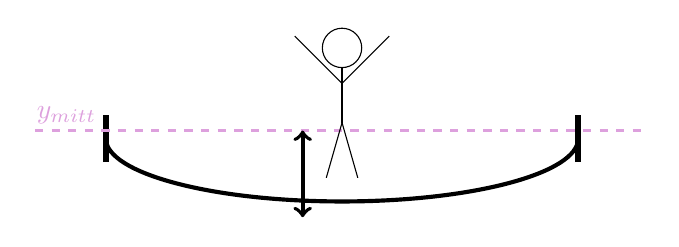
\begin{tikzpicture}

% Två raka sträck som håller i linan
\draw [line width=\size] (0,0) -- (0,\wallH);
\draw [line width=\size] (\lineW,0) -- (\lineW,\wallH);


% Själva linan
\draw [line width=1.5] (0,\wallH/2)  arc[x radius=\lineW/2, y radius=\lineH, start angle=180, end angle=360];

% Mittlinje
\draw [Plum,line width=1.2, dashed] (-0.9, 0.4) -- (\lineW+0.9,0.4);
\node [left, Plum] at (0, 0.6) {$y_{mitt}$};

% Ben
\draw (\lineW/2-0.2,-0.2) -- (\lineW/2,0.5);
\draw (\lineW/2+0.2,-0.2) -- (\lineW/2,0.5);

% Kropp
\draw (\lineW/2,0.5) -- (\lineW/2,1.2);

% Armar
\draw (\lineW/2-0.6,1.6) -- (\lineW/2,1);
\draw (\lineW/2+0.6,1.6) -- (\lineW/2,1);

% Huvud
\draw (\lineW/2, 1.45) circle [radius=0.25];


% Pil
\draw [<->, line width=1.4] (\lineW/2-0.5, 0.4) -- (\lineW/2-0.5, -0.7);


\end{tikzpicture}}
    \caption{En person på en lina i jämviktsläge}    
    \label{fig:skiss}
\end{figure}

\newpage\subsection{Modell}

\begin{figure}[h] % h = here
    \centering
    \newcommand{\wallH}{0.6} % = wall height
\newcommand{\lineW}{6} % = line width
\newcommand{\lineH}{0.8} % = line height diff
\newcommand{\size}{2.3} % Tjocklek på linjerna

\newcommand{\arrow}{1.5} % Tjocklek på pilarna

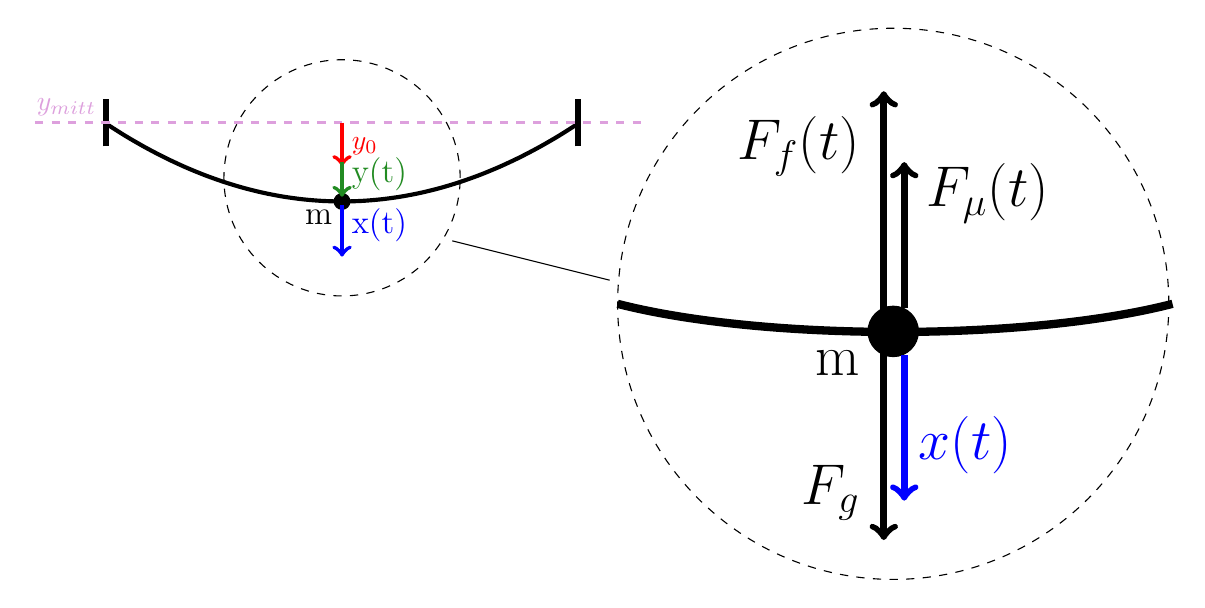
\begin{tikzpicture}

% Två raka sträck som håller i linan
\draw [line width=\size] (0,0) -- (0,\wallH);
\draw [line width=\size] (\lineW,0) -- (\lineW,\wallH);


% Själva linan
%\draw [line width=1.5] (0,\wallH/2)  arc[x radius=\lineW/2, y radius=\lineH, start angle=180, end angle=360];
%\draw [line width=1.5] (0,\wallH/2) arc (180:360:\lineW/2 and \lineH);
\draw [line width=1.5, domain=0:\lineW, smooth, variable=\x] plot ({\x},{-0.7+ 0.11*(\x-\lineW/2)*(\x-\lineW/2)});

% Mittlinje
\draw [line width=1.2, dashed, Plum] (-0.9,0.3) -- (\lineW+0.9,0.3);
\node [left, Plum] at (0, 0.5) {$y_{mitt}$};

% punkt m
\draw [fill] (\lineW/2, -0.7) circle [radius=0.1];
\node [left] at (\lineW/2, -0.9) {\large m};

% y_0
\draw [->, line width=\arrow, red] (\lineW/2, 0.3) -- (\lineW/2,-0.25);
\node [right, red] at (\lineW/2, 0) {$y_{0}$};

% y(t)
\draw [->, line width=\arrow, ForestGreen] (\lineW/2, -0.2) -- (\lineW/2, -0.64);
\node [right, ForestGreen] at (\lineW/2, -0.35) {\large y(t)};

% x(t)
\draw [->, line width=\arrow, Blue] (\lineW/2, -0.75) -- (\lineW/2, -1.4);
\node [right, Blue] at (\lineW/2, -1) {\large x(t)};

% d
%\node [centered] at (1.5, -1.1) {\large d};
%\draw [<->, line width=1] (0, -0.8) -- (3, -0.8);

% liten zoom-cirkel
\draw [dashed] (\lineW/2, -0.4) circle [radius=1.5];

% stor zoom-cirkel
\draw [dashed] (\lineW + 4, -2) circle [radius=3.5];

% linje mellan cirklarna
\draw (4.4, -1.2) -- (6.4,-1.7);

% stor lina
\draw [line width=3]  (6.5,-2) arc (220:320:4.6 and 1);

% stor Refenslinje
%\draw [line width=1.2, dashed, red] (7.1,-3.9) -- (12.95,-3.9);

% stor Mittlinje
%\draw [line width=1.2, dashed, Plum] (6.6,-1.1) -- (13.4,-1.1);

% stor punkt
\draw [fill] (10, -2.35) circle [radius=0.32];

% stort m
\node [left] at (9.7, -2.75) {\huge m};

% kraft: f
\draw [->, line width=2.5] (9.88, -2.35) -- (9.88, 0.7);
\node [left] at (9.7, 0) {\huge $F_{f}(t)$};

% kraft: g
\draw [->, line width=2.5] (9.88, -2.35) -- (9.88, -5);
\node [left] at (9.7, -4.4) {\huge $F_g$};

% stor x(t)
\draw [->, line width=2.5, Blue] (10.14, -2.65) -- (10.14, -4.5);
\node [right, Blue] at (10.2, -3.8) {\huge $x(t)$};

% kraft: my
\draw [<-, line width=2.5] (10.14, -0.2) -- (10.14, -2.05);
\node [right] at (10.3, -0.6) {\huge $F_{\mu}(t)$};

% Fs1
%\draw [->, line width=2.5] (9.88, -2.35) -- (6.88, -0.8);
%\node [right] at (6.6, -1.7) {\Large $F_{s1}(t)$};

% Fs2
%\draw [->, line width=2.5] (10.14, -2.35) -- (13.22, -0.8);
%\node [left] at (13.4, -1.7) {\Large $F_{s2}(t)$};

\end{tikzpicture}
    \caption{Modell av systemet med utritade krafter och riktningar}
    \label{fig:modell}
\end{figure}

Lindansaren modelleras som en punktformad massa $m$ som sitter i mitten på linan (se Figur \ref{fig:modell}). 
Denna massa kommer då röra sig vertikalt när den påverkas av krafter.
Den lila streckade horisontallinjen $y_{mitt}$ är systemets referensnivå och utgör en linje mellan linans fästpunkter. $y_0$ är avståndet från referensnivån $y_{mitt}$ då systemet är i vila.

\subsection{Insignal och utsignal}
\textbf{Insignal} $\bm{x(t)}$:
en kraft applicerad på massan $m$ i lodrät rikning med positiv riktning nedåt.

\textbf{Utsignal} $\bm{y(t)}$:
en distansavvikelse från $y_0$. Positiv riktning nedåt.

\subsection{Krafter}
För att modellera systemet korrekt är det viktigt att beskriva alla involverade krafter som verkar på $m$ (se Figur 2). Nedan följer dessa kraftbeskrivningar.

$\bm{F_g}$ är tyngdkraften och beskrivs enligt: 
$$F_g=mg$$
där $g$ är tyngdaccelerationen. Denna kraft beror inte på positionen av punktmassan och är tidsoberoende.

$\bm{F_f(t)}$ är systemets fjäderkraft. Linan påverkar massan $m$ med $F_f(t)$ på grund av spänningskrafter i linan vars resultant pekar i vertikal riktning. Enligt Hookes lag är denna kraft motriktad och proportionell mot massan $m$:s förflyttning från referensnivån $y_{mitt}$. Eftersom fjäderkraften är motriktad förflyttningen definerar vi positiv riktning för $F_f(t)$ uppåt. Massan $m$:s förflyttning från $y_{mitt}$ kan beskrivas som $y_0+y(t)$. Fjäderkraften kan alltså beskrivas som: $$F_f(t) = k(y_0+y(t))$$

$\bm{F_\mu(t)}$ är en friktionskraft som uppkommer på grund av friktion i linan samt luftmotståndet. Denna kraft kan antas vara modelerbar som en viskös dämpningskraft.En viskös dämpningskraft motverkar hastigheten. Eftersom hastigheten är förstaderivatan av positionen kan denna kraft beskrivas enligt: 
$$F_\mu(t) = c\frac{dy(t)}{dt}$$
där $c$ är någon friktionskonstant och positiv riktning för $F_\mu(t)$ är uppåt.

\subsection{Differentialekvation}
Den resulterande kraften som verkar på $m$ kan skrivas som summan av alla krafter som verkar på $m$. Vi summerar krafterna med positiv riktning nedåt. Detta gör att krafter definerade med positiv riktning uppåt (se Figur 2) subtraheras. Enligt Newtons andra lag kan den resulterande kraften även skrivas som massan multiplicerat med accelerationen, varpå accelerationen kan uttryckas som lägets andraderivata. Då dessa är ekvivalenta kan vi skriva:

$$m\frac{d^{2}y(t)}{dt^{2}} = x(t) - F_\mu(t) - F_f(t) + F_g$$

Med insättning av uttrycken för $F_\mu(t)$, $F_f(t)$ och $F_g$ samt omflyttning av ekvationen så att alla termer som innehåller $y(t)$ finns i vänsterled och $x(t)$ finns i högerled fås: 

\begin{equation}
m\frac{d^{2}y(t)}{dt^{2}} + c\frac{dy(t)}{dt} + k(y_{0}+y(t)) - mg=x(t)    
\end{equation}

I viloläget gäller: 
$$x(t) = y(t) = \frac{dy(t)}{dt} = \frac{d^{2}y(t)}{dt^{2}} = 0 $$

Vid insättning av dessa värden i (1) fås:
$$ky_{0} - mg = 0$$

vilket ger följande differentialekvation:

\begin{center}
    \framebox[1.1\width]{$m\displaystyle\frac{d^2y(t)}{dt^2} + c\displaystyle\frac{dy(t)}{dt} + ky(t)=x(t)$} 
    \par
\end{center}
Differentialekvationen ovan beskriver förhållandet mellan insignalen $x(t)$ och utsignalen $y(t)$. 
Denna differentialekvation kommer längre fram i rapporten tillsammans med Laplacetransformen användas för att beskriva diverse systemegenskaper. 

\subsection{Linjäritet}
För att systemet som vi har valt ska vara ett LTI system måste det vara linjärt och tidsinvariant. I denna rapport kommer vi inte visa att systemet är tidsinvariant men vi kommer visa att systemet är linjärt. För att kunna visa detta behöver vi först definiera vad som menas med att system är linjärt. Detta innebär att den ska uppfylla två kriterier: systemet ska vara additivt och det ska vara homogent.

Betrakta ett system där godtyckliga insignaler $x_1(t)$ och $x_2(t)$ ger upphov till utsignalerna $y_1(t)$ respektive $y_2(t)$. För att ett sådant system ska vara additivt måste den sammansatta insignalen $x(t)=x_1(t)+x_2(t)$ ge upphov till utsignalen $y(t)=y_1(t)+y_2(t)$.

Att ett system är homogent innebär att en insignal till systemet multiplicerat med en konstant ger upphov till en utsignal multiplicerat med samma konstant. Det vill säga om en insignal $x(t)$ till systemet ger upphov till en utsignal $y(t)$, ger insignalen $ax(t)$ upphov till utsignalen $ay(t)$, där a är en godtycklig konstant.

\subsection{Bevis av linjäritet}
För att visa att ett system är linjärt behöver man visa att det uppfyller båda kriterierna som presenterats ovan. 
Givet att insignalerna $x_1(t)$ och $x_2(t)$ ger utsignalerna $y_1(t)$ respektive $y_2(t)$ så kan man bevisa att båda kriterierna uppfylls  genom att visa att insignalen $ax_1(t) + bx_2(t)$ ger utsignalen $ay_1(t) + by_2(t)$, där a och b är godtyckliga konstanter.

Här utnyttjas att $x(t)$  kan bytas ut till differentialekvationen ovan samt det faktum att derivator är linjära.
\begin{equation*} \label{eq1.6a}
\begin{split}
x(t)
&=ax_1(t)+bx_2(t)\\
&=a\left(m\frac{d^2y_1(t)}{dt^2}+c\frac{dy_1(t)}{dt}+ky_1(t)\right)+b\left(m\frac{d^2y_2(t)}{dt^2}+c\frac{dy_2(t)}{dt}+ky_2(t)\right)\\
&=m\frac{d^2(ay_1(t)+by_2(t))}{dt^2}+c\frac{d(ay_1(t)+by_2(t))}{dt}+k(ay_1(t)+by_2(t))\\
&=m\frac{d^2y(t)}{dt^2}+c\frac{dy(t)}{dt}+ky(t)\\
\end{split}
\end{equation*} 


där $y(t)=ay_1(t)+by_2(t)$. $\blacksquare$

Man ser att insignaler kan slås ihop så att de bildar en ihopslagen utsignal av systemet. Exempelvis är det helt ekvivalent att slänga två 5 kg vikter samtidigt till lindansare som att slänga en vikt på 10 kg.
 

